\documentclass[]{article}

% Imported Packages
%------------------------------------------------------------------------------
\usepackage{amssymb}
\usepackage{amstext}
\usepackage{amsthm}
\usepackage{amsmath}
\usepackage{enumerate}
\usepackage{fancyhdr}
\usepackage[margin=1in]{geometry}
\usepackage{graphicx}
\usepackage{extarrows}
\usepackage{setspace}
\usepackage{float}
\usepackage{longtable}
% \newcommand{\tableitem}{~~\llap{\textbullet}~~}

%------------------------------------------------------------------------------

% Header and Footer
%------------------------------------------------------------------------------
\pagestyle{fancy}  
\lhead{T2 Group 10}
\chead{High-Level Architectural Design}
\rhead{SFWRENG 3A04}
\renewcommand\headrulewidth{0.4pt}                  
\renewcommand\footrulewidth{0.4pt}                                   
%------------------------------------------------------------------------------

% Title Details
%------------------------------------------------------------------------------
\title{\textbf{Boardzilla\break High-Level Architectural Design}}
\author{Matthew Paulin \\ paulinm \\ 400187147 \and
        Hargun Bedi \\ bedih \\ 400185463 \and
        Dylan Smith \\ smithd35 \\ 001314410 \and
        Chenwei Song \\ songc12 \\ 400124879 \and
        Tianzheng Mai \\ mait6 \\ 400143042
}
\date{\today}                             
%------------------------------------------------------------------------------

% Document
%------------------------------------------------------------------------------
\begin{document}

\maketitle	
\newpage
\tableofcontents
\newpage
\section{Introduction}
\label{sec:introduction}
% Begin Section

% This section should provide an brief overview of the entire document.

\subsection{Purpose}
\label{sub:purpose}
% Begin SubSection
High-level architectural design will provide an overview of the design of the entire system by identifying and delineating responsibilities of the system's components and all the interactions between them. The document's aim is to allow the stakeholders to not only understand the architectural design of the system, but also obtain a justification for why a particular design was chosen. The target audience includes the professor and teaching assistants who will inspect the document as well as the developers who may use this document as a reference.
% \begin{enumerate}[a)]
% 	\item Delineate the purpose of the document
% 	\item Specify the intended audience for the document
% \end{enumerate}
% End SubSection


\subsection{System Description}
\label{sub:system_description}
% Begin SubSection
The system that will be outlined in this document is called Boardzilla. Boardzilla is an online application that serves as a dashboard for a variety of information meant to serve as a daily briefing or hub. Each user will have their own protected account with a customizable dashboard screen containing the widgets of their choice. The users are able to select their desired amounts of a weather widget, a sticky notes widget, a calendar widget, a stock widget and a news widget. Widgets can be added or removed and can be repositioned on the users' dashboards. In addition, users will be able to input data into each widget and modify options unique to each widget.
% \begin{enumerate}[a)]
% 	\item Give a brief description of the system. This could be a paragraph or two to give some context to this document.
% \end{enumerate}
% End SubSection

\subsection{Overview}
\label{sub:overview}
% Begin SubSection
After this introduction, the document will contain a detailed outline of the architectural design. It will begin with section two, an Analysis Class Diagram, describing how each of the system's components interact with each other. This diagram will also show the hierarchical relationship between components. Section three, Architectural Design, provides a description of the system's chosen architecture as well as a justification for this choice. It will also demonstrate how each component fits into the described architecture. The responsibilities of each of these components is then described in further detail in the fourth section, Class Responsibility Collaboration (CRC) Cards. Each card will detail the responsibilities of a single component and will name the collaborating components. The last section is a division of labour that details how the production of this document was split among group members.   
% \begin{enumerate}[a)]
% 	\item Describe what the rest of the document contains 
% 	\item Explain how the document is organised
% \end{enumerate}
% End SubSection

% End Section
\newpage
\section{Analysis Class Diagram}
\label{sec:analysis_class_diagram}
% Begin Section
\begin{figure}[!ht]
\begin{center}
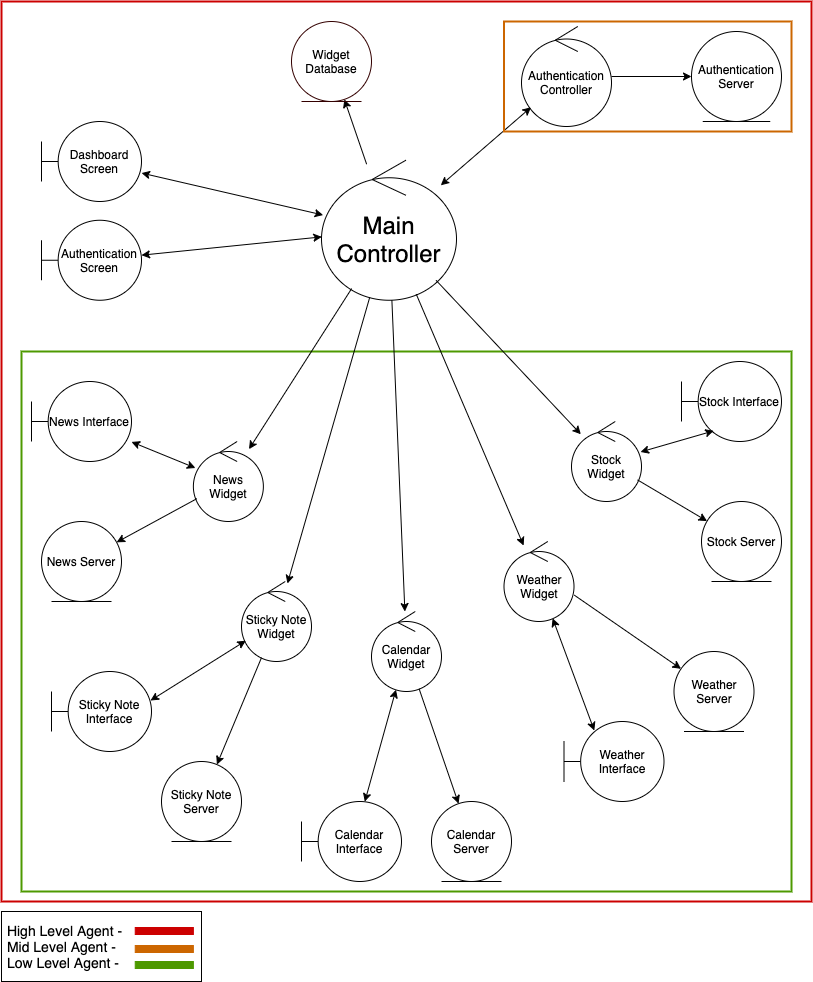
\includegraphics[width=0.95\textwidth]{ACD.png}
\end{center}
\caption{ACD Diagram}
\label{fig:Analysis Class diagram}
\end{figure}

\section{Architectural Design}
\label{sec:architectural_design}
% Begin Section
% This section should provide an overview of the overall architectural design of your application. You overall architecture should show the division of the system into subsystems with high cohesion and low coupling.
\subsection{System Architecture}
\label{sub:system_architecture}
% Begin SubSection
The overall architecture for this system is the Presentation Abstraction Control (PAC) architecture. This architecture is a more complicated version of the Model View Controller (MVC) architecture. Each agent is separated into a triplet of a Presentation, an Abstraction, and a Control component. These agents are then organized hierarchically with communication between them being facilitated by the Control components of each triad. Similarly to the MVC architecture, the user interface elements are displayed solely through the Presentation components which obtain their information from the Abstraction. The Abstraction is like the Model in MVC, but may only contain some of the over-arching data structure of the system. It does not actively notify components or agents of changes to the data because the Control components handle this functionality. The Control components also process external events and adjust the stored data accordingly.
\\
\\
Our system represents the PAC architecture as a consequence of the hierarchy of the agents which are mostly comprised of PAC triplets. The system contains low level independent agents, the different widgets, that each provide different functionalities, have different interfaces and store their own data. This necessitates the need for every agent to have their own Presentation for the corresponding user interfaces, Abstraction for data storage, and Control to facilitate inter and intra-agent communication. Due to their differences, the widgets do not need to communicate with one another, thus all communication between high and low level agents is done through the main controller, the high level agent. All the widgets exist in parallel which allows users to view and interact with the interface of any of them at any given time. This architecture is ideal because we want the users to be able to view and interact with each of their widgets on the same screen. This parallelism is one of the major reasons we chose a PAC design over the MVC pattern. In addition, the PAC architecture's modular design makes it very easy to add different widgets without modifying any of the others, following the principal of information hiding. Additionally, the separation of the agents allows for some performance benefits due to the lack of a monolithic model. 

% \large {\textbf{need to make boxes of different color around each agent in the ACD to better show the hierarchy (d) }}

% \begin{enumerate}[a)]
% 	\item Identify and explain the overall architecture of your system
% 	\item Be sure to clearly state the name of the architecture
% 	\item Provide the reasoning and justification of the choice
% 	\item Provide a structural architecture diagram showing the relationship among the subsystems (if appropriate)
% \end{enumerate}
% End SubSection

\subsection{Subsystems}
\label{sub:subsystems}

The high level agent includes the Main Controller, the Authentication and Dashboard screens the Widget database. The controller corresponds to the Control component, the two screens constitute the Presentation of the agent, and the database represents the Abstraction. Interactions between the Abstraction and Presentation components is facilitated by the Main Controller. Connected to this agent are five low level widget agents as well as an authentication agent for managing authenticated sessions. Communication between these agents and the high level agent is also done through the Main Controller. 
The Dashboard Screen is the principal interface of this agent and displays all of the users widgets in the users' chosen layout. The addition, removal, or repositioning of the widget is communicated from the dashboard to the Widget Database through the controller. The dashboard will enable the user to logout, causing the controller to send data to the Authentication controller to invalidate a user's session. The secondary Presentation is the Authentication Screen and is responsible for displaying the user interface corresponding to the login, registration and password reset screens. User inputs are communicated to the Authentication Controller through the Main controller. The Main Controller also transfers control to the low level agents when necessary to update the displayed widgets or to enable user interaction with particular widgets.
\\ \\
The authentication agent is a unique subsystem in that it is the one agent that is not comprised of a PAC triplet. This is because there is no need for a display at this level in the hierarchy. Instead, the Presentation component is handled by the main controller, high level agent, which can more easily switch presentations between the Authentication Screen and the Dashboard Screen. The Authentication Controller is the Control component and the Authentication Server is the Abstraction.
This agent is responsible for communicating user inputted authentication data to the Authentication Server as well as retrieving data from the server to validate and keep track of user sessions. The data from the server is then sent to the main controller, where the presentations can be adjusted accordingly.
\\ \\
The low level agents are all PAC triplets corresponding to one of five different widget subsystems. Each agent has a particular user interface so every Presentation component uniquely displays widget data. Since there can be multiple of each type of widget, at one time, there may be multiple Presentation components corresponding to the same agent. In addition, users can interact with the agents to modify the data displayed as well as other widget settings. Each widget will differ in what can be modified by the user. Relevant widget data is retrieved from the Abstraction, represented by different widget servers and is then sent to the Presentation through the Control. Similarly, all updated widget data is reflected in the Abstractions through communication from the presentation through the Control components. The low level agents do not communicate with one another at all, but receive communication from the high level agent when given control or asked to surrender it.



% End Section
\section{Class Responsibility Collaboration (CRC) Cards}
\label{sec:class_responsibility_collaboration_crc_cards}
% Begin Section
\begin{longtable}{| p{.70\textwidth} | p{.30\textwidth} |}
	\hline
	\multicolumn{2}{|l|}{\textbf{Class Name: Main Controller}} \\
	\hline
	\textbf{Responsibility:} & \textbf{Collaborators:} \\
	\hline
	\begin{itemize}
	    \item Interacts with Dashboard Screen to display the users' widgets in their locations when their session is validated
	    \item Uses the controllers of the widgets to display the widget information
	    \item Passes control to the controllers corresponding to the widget that the user interacts with (News Widget, Sticky Note Widget, Calendar Widget, Weather Widget, Stock Widget)
	    \item Interacts with the Widget Database to save widgets' positions
	    \item Update references to widgets in the Widget Database if they are added or deleted on the user's dashboard
		\item Interact with Authentication Controller to invalidate the session upon user logout
		\item Interact with Authentication Controller to validate a session upon user login
		\item Interacts with Authentication Screen to get user login
		\item Interacts with Authentication Screen to obtain user registration data
		\item Interacts with the Authentication Controller to reset a user's password
		\item Interacts with Authentication Screen to display an error message for invalid inputs or incorrect credentials
		\item Interacts with Authentication Screen to display a success message upon password change or user registration
    \end{itemize} & 
	\begin{itemize}
		\item Dashboard Screen
        \item Authentication Screen
        \item Widget Database
        \item Authentication Controller
		\item News Widget
		\item Calendar Widget
		\item Weather Widget
		\item Stock Widget
		\item Sticky Note Widget
	\end{itemize} \\
	\hline
	\caption{CRC for Main Controller}
\end{longtable}
\newpage
\begin{longtable}{| p{.70\textwidth} | p{.30\textwidth} |}
	\hline
	\multicolumn{2}{|l|}{\textbf{Class Name: Dashboard Screen}} \\
	\hline
	\textbf{Responsibility:} & \textbf{Collaborators:} \\
	\hline
	\begin{itemize}
		\item Allows users to add and delete widgets
		\item Enable users to reposition widgets and minimize them
		\item Send updated widget statuses to the Main Controller
		\item Display widgets in accordance with the user's saved layout
		\item Interacts with the Main controller to allow the users to log out 
    \end{itemize} & 
	\begin{itemize}
		\item Main Controller
	\end{itemize} \\
	\hline
	\caption{CRC for Dashboard Screen}
\end{longtable}

\begin{longtable}{| p{.70\textwidth} | p{.30\textwidth} |}
	\hline
	\multicolumn{2}{|l|}{\textbf{Class Name: Authentication Screen}} \\
	\hline
	\textbf{Responsibility:} & \textbf{Collaborators:} \\
	\hline
	\begin{itemize}
		\item Allows users to log in to their account with valid credentials.
		\item Allows users to register a new account by entering a valid username and password.
		\item Allows users to reset password if they have an existing account.
		\item Display an error message after user submits invalid credentials for login, registration, or password modification
		\item Display a success message upon password change or registration
    \end{itemize} & 
	\begin{itemize}
		\item Main Controller
	\end{itemize} \\
	\hline
	\caption{CRC for Authentication Screen}
\end{longtable}

\begin{longtable}{| p{.70\textwidth} | p{.30\textwidth} |}
	\hline
	\multicolumn{2}{|l|}{\textbf{Class Name: Widget Database}} \\
	\hline
	\textbf{Responsibility:} & \textbf{Collaborators:} \\
	\hline
	\begin{itemize}
		\item Stores a reference to the identity of all widgets
		\item Stores users' widget positioning data
    \end{itemize} & \newline \newline N/A \\
	\hline
	\caption{CRC for Widget Database}
\end{longtable}
\newpage
\begin{longtable}{| p{.70\textwidth} | p{.30\textwidth} |}
	\hline
	\multicolumn{2}{|l|}{\textbf{Class Name: Authentication Controller}} \\
	\hline
	\textbf{Responsibility:} & \textbf{Collaborators:} \\
	\hline
	\begin{itemize}
		\item Interact with Authentication Server to check if the session is authenticated
	    \item Interact with Main Controller to invalidate the session if the user attempts to log out
	    \item Interact with the Main Controller to validate the session upon login or registration
	    \item Interact with Main Controller to notify if the credentials entered are valid logins or registrations
		\item Interact with the Authentication Server to store the registered credentials
		\item Interact with Main Controller to notify if the account has registered successfully
		\item Interact with the Authentication Server to verify login attempts
		\item Interact with the Main Controller to redirect the user to the Dashboard Screen upon login or registration 
		\item Interact with Main Controller to notify if the password has been changed successfully
		\item Interact with Authentication Server to store the reset credentials
    \end{itemize} & 
	\begin{itemize}
	    \item Main Controller
		\item Authentication Server
	\end{itemize} \\
	\hline
	\caption{CRC for Authentication Controller}
\end{longtable}

\begin{longtable}{| p{.70\textwidth} | p{.30\textwidth} |}
	\hline
	\multicolumn{2}{|l|}{\textbf{Class Name: Authentication Server}} \\
	\hline
	\textbf{Responsibility:} & \textbf{Collaborators:} \\
	\hline
	\begin{itemize}
		\item Stores login credentials
		\item Stores references to valid user sessions
    \end{itemize} & 
	\begin{itemize}
		\item Authentication Controller
	\end{itemize} \\
	\hline
	\caption{CRC for Authentication Server}
\end{longtable}
\newpage
\begin{longtable}{| p{.70\textwidth} | p{.30\textwidth} |}
	\hline
	\multicolumn{2}{|l|}{\textbf{Class Name: News Widget}} \\
	\hline
	\textbf{Responsibility:} & \textbf{Collaborators:} \\
	\hline
	\begin{itemize}
		\item Interact with the News Server to get updated news data in accordance with the widgets' settings
		\item Interact with News Interface to display the news contents.
		\item Interact with the News Interface to get user inputted widget settings
		\item Interact with the News Server to store updated settings
    \end{itemize} & 
	\begin{itemize}
		\item News Interface
        \item News Server
	\end{itemize} \\
	\hline
	\caption{CRC for News Widget}
\end{longtable}

\begin{longtable}{| p{.70\textwidth} | p{.30\textwidth} |}
	\hline
	\multicolumn{2}{|l|}{\textbf{Class Name: News Interface}} \\
	\hline
	\textbf{Responsibility:} & \textbf{Collaborators:} \\
	\hline
	\begin{itemize}
		\item Display news data in accordance with the widgets' settings
		\item Allow users to modify widget settings
		\item Enables users to choose news topics
		\item Interact with News Widget to send updated settings
    \end{itemize} & 
	\begin{itemize}
		\item News Widget
	\end{itemize} \\
	\hline
	\caption{CRC for News Interface}
\end{longtable}

\begin{longtable}{| p{.70\textwidth} | p{.30\textwidth} |}
	\hline
	\multicolumn{2}{|l|}{\textbf{Class Name: News Server}} \\
	\hline
	\textbf{Responsibility:} & \textbf{Collaborators:} \\
	\hline
	\begin{itemize}
		\item Store News data
		\item Acquires updated News data
		\item Stores widget settings
    \end{itemize} & \newline \newline  N/A \\
	\hline
	\caption{CRC for News Server}
\end{longtable}
\newpage
\begin{longtable}{| p{.70\textwidth} | p{.30\textwidth} |}
	\hline
	\multicolumn{2}{|l|}{\textbf{Class Name: Calendar Widget}} \\
	\hline
	\textbf{Responsibility:} & \textbf{Collaborators:} \\
	\hline
	\begin{itemize}
        \item Acquires Calendar information from the Calendar Server in accordance with the widgets' settings
		\item Interact with Calendar Interface to display the widget contents.
		\item Interact with the Calendar Interface to get user inputted widget settings
		\item Interact with the Calendar Interface to get user input
		\item Interact with the Calendar Server to store changes to calendar
		\item Interact with the Calendar Server to store widget settings
    \end{itemize} & 
	\begin{itemize}
		\item Calendar Interface
        \item Calendar Server
	\end{itemize} \\
	\hline
	\caption{CRC for Calendar Widget}
\end{longtable}

\begin{longtable}{| p{.70\textwidth} | p{.30\textwidth} |}
	\hline
	\multicolumn{2}{|l|}{\textbf{Class Name: Calendar Interface}} \\
	\hline
	\textbf{Responsibility:} & \textbf{Collaborators:} \\
	\hline
	\begin{itemize}
		\item Display calendar data in accordance with the widgets' settings
		\item Allow users to modify widget settings
		\item Allow user to add events to their calendar
		\item Allow user to toggle between calendar views
		\item Interact with Calendar Widget to send updated settings
    \end{itemize} & 
	\begin{itemize}
		\item Calendar Widget
	\end{itemize} \\
	\hline
	\caption{CRC for Calendar Interface}
\end{longtable}

\begin{longtable}{| p{.70\textwidth} | p{.30\textwidth} |}
	\hline
	\multicolumn{2}{|l|}{\textbf{Class Name: Calendar Server}} \\
	\hline
	\textbf{Responsibility:} & \textbf{Collaborators:} \\
	\hline
	\begin{itemize}
		\item Store Calendar data
		\item Acquires updated Calendar data
		\item Stores widget settings
    \end{itemize} & \newline \newline  N/A \\
	\hline
	\caption{CRC for Calendar Server}
\end{longtable}
\newpage
\begin{longtable}{| p{.70\textwidth} | p{.30\textwidth} |}
	\hline
	\multicolumn{2}{|l|}{\textbf{Class Name: Weather Widget}} \\
	\hline
	\textbf{Responsibility:} & \textbf{Collaborators:} \\
	\hline
	\begin{itemize}
		\item Interact with the Weather Server to get updated weather data in corresponding to the widgets' settings
		\item Interact with Weather Interface to display the widget contents.
		\item Interact with the Weather Interface to get user inputted widget settings
		\item Interact with the Weather Server to store updated settings 
    \end{itemize} & 
	\begin{itemize}
		\item Weather Interface
        \item Weather Server 
	\end{itemize} \\
	\hline
	\caption{CRC for Weather Widget}
\end{longtable}

\begin{longtable}{| p{.70\textwidth} | p{.30\textwidth} |}
	\hline
	\multicolumn{2}{|l|}{\textbf{Class Name: Weather Interface}} \\
	\hline
	\textbf{Responsibility:} & \textbf{Collaborators:} \\
	\hline
	\begin{itemize}
		\item Display weather data corresponding to the widgets' settings
		\item Allow users to modify weather location
		\item Allows users to toggle between various weather data
		\item Interact with Weather Widget to send updated settings
    \end{itemize} & 
	\begin{itemize}
		\item Weather Widget
	\end{itemize} \\
	\hline
	\caption{CRC for Weather Interface}
\end{longtable}

\begin{longtable}{| p{.70\textwidth} | p{.30\textwidth} |}
	\hline
	\multicolumn{2}{|l|}{\textbf{Class Name: Weather Server}} \\
	\hline
	\textbf{Responsibility:} & \textbf{Collaborators:} \\
	\hline
	\begin{itemize}
		\item Store weather data.
		\item Acquires updated weather data
		\item Stores widget settings
    \end{itemize} & \newline \newline  N/A \\
	\hline
	\caption{CRC for Weather Server}
\end{longtable}
\newpage
\begin{longtable}{| p{.70\textwidth} | p{.30\textwidth} |}
	\hline
	\multicolumn{2}{|l|}{\textbf{Class Name: Stock Widget}} \\
	\hline
	\textbf{Responsibility:} & \textbf{Collaborators:} \\
	\hline
	\begin{itemize}
		\item Interact with the Stock Server to get updated stock data in accordance with the widget settings
		\item Interact with Stock Interface to display the stock data.
		\item Interact with the Stock Interface to get user inputted stock settings
		\item Interact with the Stock Server to store users' updated stock information 
    \end{itemize} & 
	\begin{itemize}
		\item Stock Interface
        \item Stock Server
	\end{itemize} \\
	\hline
	\caption{CRC for Stock Widget}
\end{longtable}

\begin{longtable}{| p{.70\textwidth} | p{.30\textwidth} |}
	\hline
	\multicolumn{2}{|l|}{\textbf{Class Name: Stock Interface}} \\
	\hline
	\textbf{Responsibility:} & \textbf{Collaborators:} \\
	\hline
	\begin{itemize}
		\item Display stock data corresponding to the widgets' settings
		\item Allow users to select which stocks they are following
		\item Allow users to select different views that contain varying stock information
		\item Interact with Stock Widget to send updated settings
    \end{itemize} & 
	\begin{itemize}
		\item Stock Widget
	\end{itemize} \\
	\hline
	\caption{CRC for Stock Interface}
\end{longtable}

\begin{longtable}{| p{.70\textwidth} | p{.30\textwidth} |}
	\hline
	\multicolumn{2}{|l|}{\textbf{Class Name: Stock Server}} \\
	\hline
	\textbf{Responsibility:} & \textbf{Collaborators:} \\
	\hline
	\begin{itemize}
		\item Store Stock data.
		\item Acquires updated stock information
		\item Stores user stock preferences
    \end{itemize} & \newline \newline  N/A \\
	\hline
	\caption{CRC for Stock Server}
\end{longtable}
\newpage
\begin{longtable}{| p{.70\textwidth} | p{.30\textwidth} |}
	\hline
	\multicolumn{2}{|l|}{\textbf{Class Name: Sticky Note Widget}} \\
	\hline
	\textbf{Responsibility:} & \textbf{Collaborators:} \\
	\hline
	\begin{itemize}
		\item Interact with the Sticky Note Server to retrieve sticky note data and settings
		\item Interact with Sticky Note Interface to display users' sticky notes.
		\item Interact with the Sticky Notes Interface to get user inputted settings
		\item Interact with the Sticky Note Server to store updated notes 
    \end{itemize} & 
	\begin{itemize}
		\item Sticky Note Interface
        \item Sticky Note Server
	\end{itemize} \\
	\hline
	\caption{CRC for Sticky Note Widget}
\end{longtable}

\begin{longtable}{| p{.70\textwidth} | p{.30\textwidth} |}
	\hline
	\multicolumn{2}{|l|}{\textbf{Class Name: Sticky Note Interface}} \\
	\hline
	\textbf{Responsibility:} & \textbf{Collaborators:} \\
	\hline
	\begin{itemize}
		\item Display user created sticky notes with their corresponding settings
		\item Allow users to modify the text on sticky notes
		\item Interact with Sticky Note Widget to save updated sticky notes
    \end{itemize} & 
	\begin{itemize}
		\item Sticky Note Widget
	\end{itemize} \\
	\hline
	\caption{CRC for Sticky Note Interface}
\end{longtable}

\begin{longtable}{| p{.70\textwidth} | p{.30\textwidth} |}
	\hline
	\multicolumn{2}{|l|}{\textbf{Class Name: Sticky Note Server}} \\
	\hline
	\textbf{Responsibility:} & \textbf{Collaborators:} \\
	\hline
	\begin{itemize}
		\item Stores sticky note data
		\item Stores sticky note settings
    \end{itemize} & \newline \newline N/A \\
	\hline
	\caption{CRC for Sticky Note Server}
\end{longtable}


% End Section
\appendix

\newpage
\section{Division of Labour}
\label{sec:division_of_labour}
% Begin Section
This document was created through a collaborative effort by the whole group, exchanging ideas and filling in sections together. Meetings were held regularly to iterate on this document until an acceptable final version was achieved. By signing this document, the group members certify that this division of labor is fair and accurate.

	\subsection{Signatures}
	\vspace{10ex}
	\begin{center}
	\noindent\begin{tabular}{ll}\\ 
	\makebox[3.5in]{\hrulefill} & \makebox[2in]	\hrulefill \\
	Matthew Paulin & Date\\[15ex]
	\makebox[3.5in]{\hrulefill} & \makebox[2in]	\hrulefill \\		
	Hargun Bedi & Date\\[15ex]
	\makebox[3.5in]{\hrulefill} & \makebox[2in]	\hrulefill \\		
	Dylan Smith & Date\\[15ex]
	\makebox[3.5in]{\hrulefill} & \makebox[2in]	\hrulefill \\		
	Chenwei Song & Date\\[15ex]
	\makebox[3.5in]{\hrulefill} & \makebox[2in]	\hrulefill \\
	Tianzheng Mai & Date\\
	\end{tabular}
	\end{center}
% End Section

% \newpage
% \section*{IMPORTANT NOTES}
% \begin{itemize}
% %	\item You do \underline{NOT} need to provide a text explanation of each diagram; the diagram should speak for itself
% 	\item Please document any non-standard notations that you may have used
% 	\begin{itemize}
% 		\item \emph{Rule of Thumb}: if you feel there is any doubt surrounding the meaning of your notations, document them
% 	\end{itemize}
% 	\item Some diagrams may be difficult to fit into one page
% 	\begin{itemize}
% 		\item It is OK if the text is small but please ensure that it is readable when printed
% 		\item If you need to break a diagram onto multiple pages, please adopt a system of doing so and thoroughly explain how it can be reconnected from one page to the next; if you are unsure about this, please ask about it
% 	\end{itemize}
% 	\item Please submit the latest version of Deliverable 1 with Deliverable 2
% 	\begin{itemize}
% 		\item It does not have to be a freshly printed version; the latest marked version is OK
% 	\end{itemize}
% 	\item If you do \underline{NOT} have a Division of Labour sheet, your deliverable will \underline{NOT} be marked
% \end{itemize}
\end{document}
%------------------------------------------------------------------------------